\documentclass[12pt]{article}

% aprovechamiento de la p\'agina -- fill an A4 (210mm x 297mm) page

% Note: 1 inch = 25.4 mm = 72.27 pt
% 1 pt = 3.5 mm (approx)

\usepackage[paperheight=297mm,
            paperwidth=210mm,
            tmargin=13mm, 
            headheight=0mm, 
            headsep=0mm,
            textheight=276mm,
            footskip=7mm,
            textwidth=159.2mm,
            bindingoffset=10mm,
            twoside
            ]{geometry}

% paragraph setup
\setlength{\parindent}{0em}
%\setlength{\parindent}{4em}
\setlength{\parskip}{1em}
\setlength{\columnsep}{1em}
%\renewcommand{\baselinestretch}{1.5}

\usepackage{arabtex}
\usepackage{atrans}
\usepackage{nashbf}
\usepackage{twoblks}
\usepackage[utf8]{inputenc}
\usepackage[absolute]{textpos}
\usepackage{graphicx}
\usepackage[usenames,dvipsnames]{xcolor}
\usepackage{fontawesome}

\definecolor{webgreen}{rgb}{0, 0.5, 0} % less intense green
\definecolor{webblue}{rgb}{0, 0, 0.5}  % less intense blue
\definecolor{webred}{rgb}{0.5, 0, 0}   % less intense red
\usepackage[bookmarks=true,
            bookmarksnumbered=false, % true means bookmarks in 
                                     % left window are numbered                         
            bookmarksopen=false,     % true means only level 1
                                     % are displayed.
            colorlinks=true,
            linkcolor=webred,
            urlcolor=NavyBlue,
            citecolor=cyan]{hyperref}

\usepackage{tikz,everypage}
\usetikzlibrary{backgrounds}
\newcommand*{\AbsolutePosition}[3]{%
    % #1 = x (from south west corner of page)
    % #2 = y
    % #3 = content
    \AddThispageHook{%
        \begin{tikzpicture}[remember picture,overlay]
            \draw (current page.south west) ++ (#1,#2) node[opacity=0.25] {#3};%
        \end{tikzpicture}
    }
}

%%%%%%%%%%%%%%%%%%%%%%%%%%%%%%%%%%%%%%%%%%%%%%%%
%% cómo generar el código QR
%% compilar con:  pdflatex -shell-escape <file>
%% la primera vez para generar el pdf y luego 
%% comentar.
%%%%%%%%%%%%%%%%%%%%%%%%%%%%%%%%%%%%%%%%%%%%%%%%
% \usepackage{pst-barcode}
% \usepackage{auto-pst-pdf}   
%%%%%%%%%%%%%%%%%%%%%%%%%%%%%%%%%%%%%%%%%%%%%%%%%

%% selección de la fuente global
\usepackage[
            light,
            math]
           {kurier}
\usepackage[T1]{fontenc}

\pagestyle{empty}

\begin{document}

\pagestyle{empty}
\tracingarab=0
\setarab
\settrans{spanish}
\novocalize
\arabtrue

% %\begin{textblock*}{290mm}(185mm,258mm)
% \begin{textblock*}{290mm}(25mm,2mm) % Granada y Motril
% %\begin{textblock*}{290mm}(25mm,4mm) % Sevilla
%   \includegraphics[scale=1]{taqwim.pdf}
% \end{textblock*}

\begin{center}
\href{http://bcnmosque.com/}{\Huge\textsc{Fundación Mezquita de Barcelona}}
\end{center}
\AbsolutePosition{105mm}{150mm}{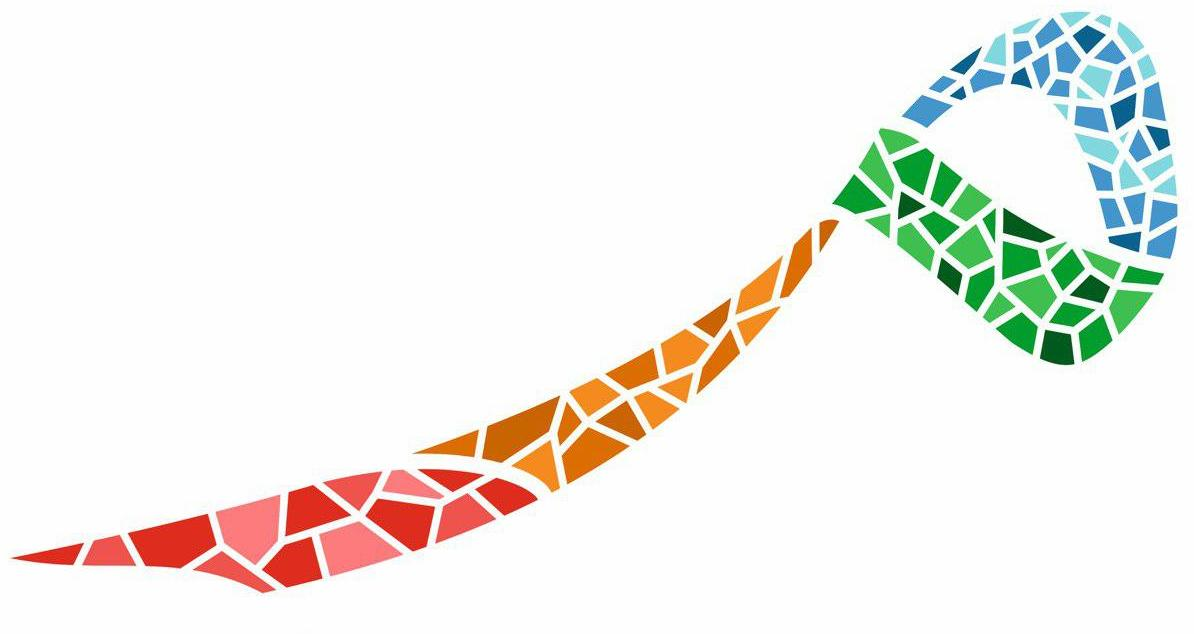
\includegraphics[scale=0.38]{mim.jpg}}

\footnotesize \twoblocks{Parte de los momentos del
  \arabfalse\transtrue \RL{.salAT} correspondiente al mes de
  \arabfalse\transtrue\settransfont{\bf\itshape} 
  mesArabTrans 
  del a\~no \textbf{agnoa h.} (agnom/agnop d.J.) para la
  ciudad de \textbf{Barcelona} y cercan\'{\i}as.  }{
  \begin{arabtext}
    \noindent
    .hi.s.saTu 'awqAti a.s-.salATi li^sahri \setnashbf 
    mAAG
    \setnash min `Ami \setnashbf <\bf agnoa> h- . \setnash(
    \LR{agnom}/\LR{agnop} m- .) limadInaTi \setnashbf bar^silUnaT
    \setnash wa-mA ^gAwarahA.
  \end{arabtext}}
\vspace{2mm}
  \normalsize
\centerline{
\begin{tabular}{|c|c|c|c|c|c|c|c|c|c|}
\hline
\RL{al-`i^sA'}&
\RL{al-ma.grib}&
\RL{al-`a.sr}&\RL{a.z-.zuhr}&
\RL{al-^surUq}&\RL{al-fa^gr}&
\multicolumn{2}{|c|}{\RL{yawmu al-'usbU`}}&
\RL{mesSolarArab2} /\RL{mesSolarArab1}&
\RL{mesArabArab}\\
\hline
\arabfalse\transtrue \RL{`i^sA'} &
\arabfalse\transtrue \RL{ma.grib}&
\arabfalse\transtrue \RL{`a.sr}  &
\arabfalse\transtrue \RL{.zuhr}  &
\arabfalse\transtrue \RL{^surUq} &
\arabfalse\transtrue \RL{fa^gr}  &
                      \multicolumn{2}{|c|}{d\'{\i}a semana}&
                      mesSolarEsp1/mesSolarEsp2  &
\settransfont{\bf\itshape}\arabfalse\transtrue
mesArabCaja\\
\hline
horario
\end{tabular}
}
                                        
\centerline{                             
\begin{tabular}{|c|c|c|c|c|c|}           
  \hline                                   
  \multicolumn{6}{|c|}{Algunos par\'ametros lunares en \textbf{Barcelona} para
    final de \arabfalse\transtrue\settransfont{\bf\itshape} 
  mesArabTrans}\\
  \hline
  d\'{\i}a de observar&
  puesta de Sol&
  puesta de Luna&
  dif. Luna-Sol&
  edad lunar&
  ?`avistamiento?\\
  \hline
  diadata&
  ssdata&
  msdata&
  smdata&
  madata&
  avdata\\ 
  \hline
\end{tabular}
}
 \vspace{2mm}

 \footnotesize \noindent \textbf{Barcelona} (41º23'N/2º09'E): longitud
 de referencia 15ºE, zona horaria +1 h, altitud sobre el nivel del mar
 25 m, \'angulo de crep\'usculo 18º, \arabfalse\transtrue \RL{qiblaT}
 110.50º, declinaci\'on dedata.

 \begin{center}
   \footnotesize
   Carrer Benet Mercadé 26 Local 1, 08012 Barcelona --- 
   Tel: +34 935 312 292\\ % --- Fax: +34 932 491 415\\
   \href{mailto:info@bcnmosque.com}{\texttt{info{@}bcnmosque.com}} ---
   \href{https://is.gd/1YNfan}{\texttt{www.bcnmosque.com}}
 \end{center}

%  
%  \centerline{\texttt{Segunda Edición}}
%  
\end{document}
